% Created 2022-03-01 Tue 15:15
% Intended LaTeX compiler: pdflatex
\documentclass[11pt]{article}
\usepackage[utf8]{inputenc}
\usepackage[T1]{fontenc}
\usepackage{graphicx}
\usepackage{longtable}
\usepackage{wrapfig}
\usepackage{rotating}
\usepackage[normalem]{ulem}
\usepackage{amsmath}
\usepackage{amssymb}
\usepackage{capt-of}
\usepackage{hyperref}
\author{David Lewis}
\date{\today}
\title{}
\hypersetup{
 pdfauthor={David Lewis},
 pdftitle={},
 pdfkeywords={},
 pdfsubject={},
 pdfcreator={Emacs 28.0.91 (Org mode 9.6)}, 
 pdflang={English}}
\begin{document}

\section*{What is Emacs?}
\label{sec:orgfb2808c}
\begin{center}

\includegraphics[width=1in]{emacs.png}
\end{center}
\subsection*{Text Editor}
\label{sec:org9e2a255}
\begin{itemize}
\item Word
\item Google docs
\item Visual Studio Code
\item Notepad
\end{itemize}
\subsection*{Text}
\label{sec:org6b3234c}
\begin{verbatim}
;; this is the emacs programming language
(message "Hello, world!")
\end{verbatim}


\begin{verbatim}
<!-- this is what the web is made of -->
<p> Here is some HTML! </p>
\end{verbatim}


\begin{verbatim}
#Markdown!
\end{verbatim}
\subsection*{What We Will Learn}
\label{sec:org6dcdaf3}
\begin{itemize}
\item What it can do
\item History
\item Philosophy
\end{itemize}
\section*{What it can do}
\label{sec:orgc09a727}
\subsection*{Edit Code}
\label{sec:orgff2bdde}
\begin{verbatim}
while True:
    print("It's an infinite loop!")

def recursion():
    print("Is this recursion?")
    return recursion()
\end{verbatim}
\subsection*{Create Documents}
\label{sec:org5b7b97a}
\begin{center}
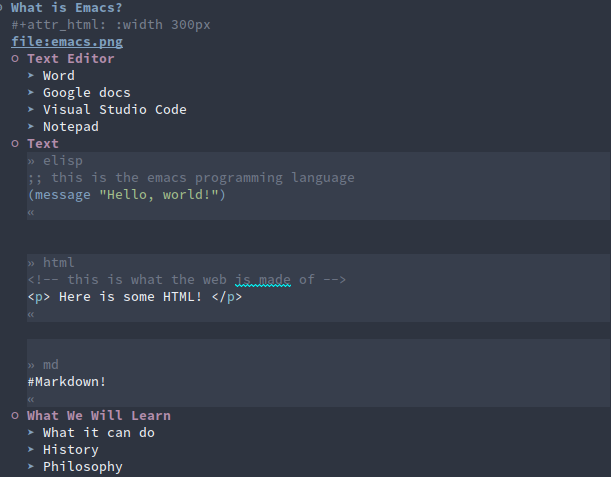
\includegraphics[width=1in]{org-mode.png}
\end{center}
\subsubsection*{This Presentation!}
\label{sec:orgefb077c}
\subsubsection*{PDF}
\label{sec:orgfba011c}
\subsubsection*{Website}
\label{sec:orgdbd241a}
\subsection*{Games}
\label{sec:orgc2afbc5}
\begin{itemize}
\item Tetris
\item Snake
\end{itemize}
\begin{center}
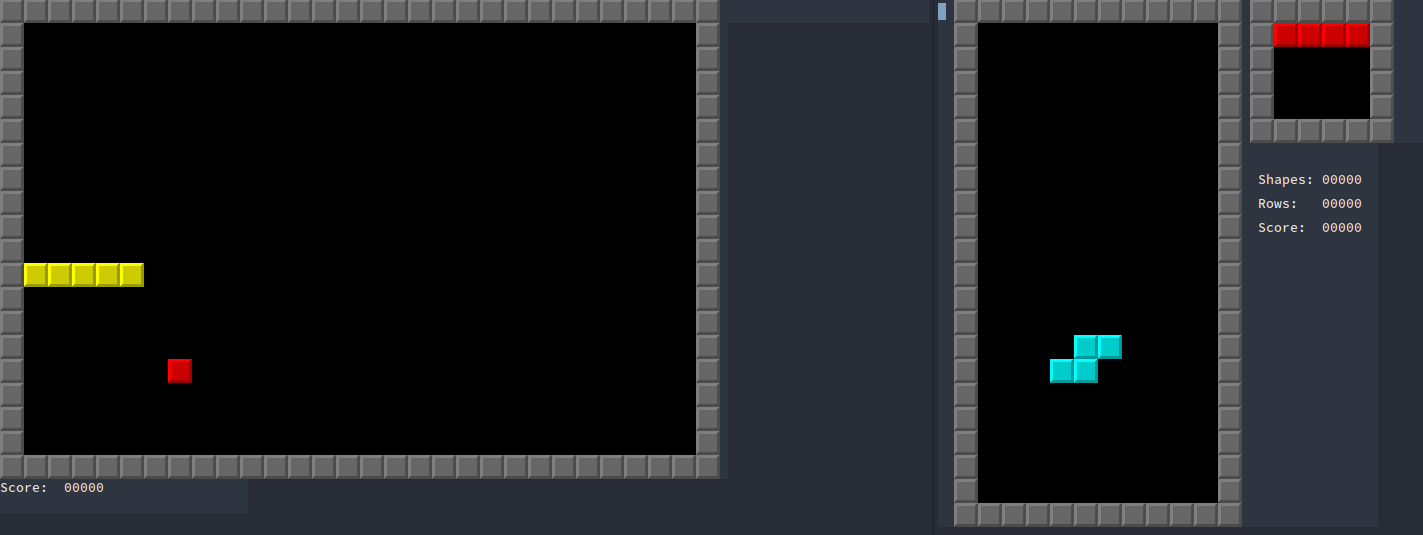
\includegraphics[width=1in]{snake.png}
\end{center}

\subsection*{Phsycologist}
\label{sec:org2591db7}
\begin{itemize}
\item Why do we exist?
\item \texttt{What do you think?}
\item Love?
\item \texttt{Can you elaborate on that?}
\item Human relationships.
\item \texttt{Why do you say human relationships?}
\item It gives live meaning.
\item \texttt{Is it because of your plans that you say it gives live meaning?}
\end{itemize}


\section*{History}
\label{sec:org7115a6a}
\begin{itemize}
\item Originally created in 1976.
\end{itemize}
\begin{center}
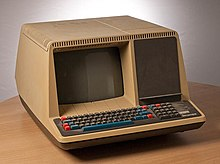
\includegraphics[width=1in]{terminal.jpg}
\end{center}
\subsection*{GNU EMACS}
\label{sec:org60c1346}
\begin{itemize}
\item First released in 1985 by Richard Stallman
\item Free and open source
\item Lisp
\end{itemize}
\begin{center}
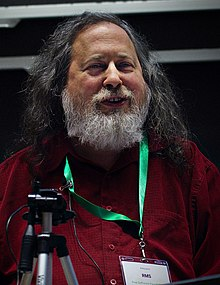
\includegraphics[width=1in]{Stallman.jpg}
\end{center}
\end{document}
